
% ===============================================
% MATH 34: Multivariable calculus           Spring 2019
% hw_template.tex
% ===============================================

% -------------------------------------------------------------------------
% You can ignore this preamble. Go on
% down to the section that says "START HERE" 
% -------------------------------------------------------------------------

\documentclass{article}

\usepackage[margin=1.5in]{geometry} % Please keep the margins at 1.5 so that there is space for grader comments.
\usepackage{amsmath,amsthm,amssymb,hyperref}
\usepackage{graphicx}
\usepackage{float}
\usepackage{listings}
\usepackage{xparse}
\usepackage{xcolor}

\newcommand{\R}{\mathbf{R}}  
\newcommand{\Z}{\mathbf{Z}}
\newcommand{\N}{\mathbf{N}}
\newcommand{\Q}{\mathbf{Q}}
\newcommand{\C}{\mathbf{C}}

\newenvironment{theorem}[2][Theorem]{\begin{trivlist}
\item[\hskip \labelsep {\bfseries #1}\hskip \labelsep {\bfseries #2.}]}{\end{trivlist}}
\newenvironment{lemma}[2][Lemma]{\begin{trivlist}
\item[\hskip \labelsep {\bfseries #1}\hskip \labelsep {\bfseries #2.}]}{\end{trivlist}}
\newenvironment{claim}[2][Claim]{\begin{trivlist}
\item[\hskip \labelsep {\bfseries #1}\hskip \labelsep {\bfseries #2.}]}{\end{trivlist}}
\newenvironment{problem}[2][Problem]{\begin{trivlist}
\item[\hskip \labelsep {\bfseries #1}\hskip \labelsep {\bfseries #2.}]}{\end{trivlist}}
\newenvironment{proposition}[2][Proposition]{\begin{trivlist}
\item[\hskip \labelsep {\bfseries #1}\hskip \labelsep {\bfseries #2.}]}{\end{trivlist}}
\newenvironment{corollary}[2][Corollary]{\begin{trivlist}
\item[\hskip \labelsep {\bfseries #1}\hskip \labelsep {\bfseries #2.}]}{\end{trivlist}}

\newenvironment{solution}{\begin{proof}[Solution]}{\end{proof}}

\makeatletter
\newcommand{\skipitems}[1]{%
	\addtocounter{\@enumctr}{#1}%
}
\makeatother

\NewDocumentCommand{\codeword}{v}{%
\texttt{\textcolor{blue}{#1}}%
}


\begin{document}

\large % please keep the text at this size for ease of reading.

% ------------------------------------------ %
%                 START HERE             %
% ------------------------------------------ %

{\Large Page 1 % Replace with appropriate page number 
\hfill  MTH483, Complex Variables, HW2}

\begin{center}
{\Large Wyatt Whiting}
\end{center}
\vspace{0.05in}

% -----------------------------------------------------
% The "enumerate" environment allows for automatic problem numbering.
% To make the number for the next problem, type " \item ". 
% To make sub-problems such as (a), (b), etc., use an "enumerate" within an "enumerate."
% -----------------------------------------------------

\begin{enumerate}
	\item Find all complex solutions of the following equations	
	\begin{enumerate}
		\item $z + 2\overline{z} = 1 \implies (a + bi) + 2(a - bi) = 1 \implies 3a - bi = 1 + 0i \implies a=\frac{1}{3}, b = 0 \implies z = \frac{1}{3} + 0i$
		\item $2z^2 + (i-1)z+5i=0 \implies z_1 = \frac{1+\sqrt{21}}{4}-\frac{1+\sqrt{21}}{4}i, z_2 = -\frac{\sqrt{21}-1}{4}+\frac{\sqrt{21}-1}{4}i$
		\item $z^2+2z^{-2}=-2 \implies z^2 +2+2z^{-2}=0\implies \frac{z^4+2z+2}{z^2}=0 \implies z^4+2z^2+2=0 \implies z_1 = 2^{1/4}e^{i\frac{5\pi}{8}}, z_2 = 2^{1/4}e^{\frac{-3\pi}{8}}, z_3=2^{1/4}e^{\frac{-5\pi}{8}}, z_4=2^{1/4}e^{\frac{3\pi}{8}}$
		\item $z^3+iz^2+7z-5i=0 \implies z_1 = i, z_2 = 0 + (\sqrt{6}-1)i, z_3 = 0-(\sqrt{6}+1)i$
	\end{enumerate}
	
	\item Find all complex roots:
	\begin{enumerate}
		\item $(i + 1)^{1/3} = z \implies z^3 = i  + 1 = \sqrt{2}\text{cis}(\frac{\pi}{4}) \implies z_1 = 2^{1/6}\text{cis}(\frac{\pi}{12}),z_2 = 2^{1/6}\text{cis}(\frac{3\pi}{4}), z_3 = 2^{1/6}\text{cis}(\frac{17\pi}{12})$
		\item $i^{1/4} = z \implies i = z^4 = \text{cis}(\frac{\pi}{2}) \implies z_1 = \text{cis}(\frac{\pi}{8}), z_2 = \text{cis}(\frac{5\pi}{8}), z_3 = \text{cis}(\frac{9\pi}{8}), z_4 = \text{cis}(\frac{13\pi}{8}) $
		
		\item $(-1)^{1/5} = z \implies -1 = z^5 = \text{cis}(\pi) \implies z_1 = \text{cis}(\frac{\pi}{5}), z_2 = \text{cis}(\frac{3\pi}{5}),z_3 = \text{cis}(\pi),z_4 = \text{cis}(\frac{7\pi}{5}),z_5 = \text{cis}(\frac{9\pi}{5})$
		
		\item $(1 + 2i)^{3/2} = z \implies z^{2/3}=1+2i \implies z^2 = (1+2i)^3=-11-2i =5\sqrt{5}\text{cis}(\arctan(2/11)) \implies z_1 = 5^{3/4}\text{cis}(\frac{\arctan{\frac{2}{11}}}{2}), z_1 = 5^{3/4}\text{cis}(\frac{\arctan{\frac{2}{11}}}{2}) $
	\end{enumerate}
	
	\item Use de Moivre's formula to express cos(3$x$) and sin(3$x$) in terms of cos($x$) and sin($x$).
	
	\[ \text{cis}^n(x)=\text{cis}(nx) \implies \text{cis}^3(x)=\text{cis}(3x) \] 
	\[ (\cos^2{x}-\sin^2{x}+2i\cos{x}\sin{x})(\cos{x}+isin{x})=\cos{3x}+i\sin{3x}\]
	\[ \cos^3{x}-3\sin^2{x}\cos{x}+i(3\cos^2{x}\sin{x}-\sin^3{x})=\cos{3x}+i\sin{3x}\]
	\[ \sin{3x}=3\cos^2{x}\sin{x}-\sin^3{x}\]
	
	\item Determine if each of the following statements is true.  If it is,  prove it.  If it is not,  give a counterexample.
	\begin{enumerate}
		\item \textit{Proof}: Let $z,w \in \C$ be arbitrary. Then $z=a+bi \text{ and } w=c+di \text{ where } a,b,c,d \in \R$. We then have $\overline{z+w}=\overline{(a+c)+i(b+d)}=(a+c)-i(b+d)=(a-ib)+(c-id)=\overline{z}+\overline{w}$. This proves $\overline{z+w}=\overline{z}+\overline{w}$.
		
		\item \textit{Proof}: Let $z,w \in \C$ be arbitrary. Then $z=a+bi \text{ and } w=c+di$ where $a,b,c,d \in \R$. We then have $\overline{zw} = \overline{(a+bi)(c+di)} =  \overline{(ac-bd)+i(ad+bc)}=(ac-bd)-i(ad+bc)=ac-iad-bd-ibc=a(c-id)-bi(c-id)=(a-bi)(c-di)=\overline{z} \thinspace \overline{w}$. This proves $ \overline{zw}= \overline{z} \thinspace \overline{w}$.
		
		\item \textit{Counterexample}: Let $z=1+0i$ and $w = 0+i$. Then $|z+w| = |1+i| = \sqrt{2}$. But $|z|=1$ and $|w|=1$ so $|z|+|w|=2\neq\sqrt{2}=|z+w|$. 
		
		\item \textit{Proof}: Let $z,w \in \C$ be arbitrary. Then $z=r_1e^{i\theta_1} \text{ and } w=r_2e^{i\theta_2}$ where $r_1,r_2 \in \R \text{ and } \theta_1,\theta_2 \in (-\pi,\pi]$. We then have $\text{Arg}(zw)=\text{Arg}(r_1r_2e^{i\theta_1+i\theta_2})=\text{Arg}(r_1r_2e^{i(\theta_1+\theta_2)})=\theta_1+\theta_2=\text{Arg}(z)+\text{Arg}(w)$. In the case that $\text{Arg}(z)+\text{Arg}(w) \notin (-\pi,\pi]$, then taking this quantity modulo 2$\pi$ will ensure it is within the range $(-\pi, \pi]$. This proves $\text{Arg}(zw)=\text{Arg}(z)+\text{Arg}(w)$ modulo 2$\pi$.
		
		\item \textit{Proof}: Let $z,w \in \C$ be arbitrary. Then $z=r_1e^{i\theta_1} \text{ and } z=r_2e^{i\theta_2}$. We then have $\text{Arg}(zw)=r_2 r_2e^{i(\theta_1+\theta_2)}$. If both $\theta_1,\theta_2 \in (\frac{-\pi}{4}, \frac{\pi}{4}]$, then $\theta_1+\theta_2\in (-\pi,\pi]$. If the sum is outside the range $(-\pi,\pi]$, then taking the quantity modulo $2\pi$ ensures it is within the range. This proves $\text{Arg}(zw)=\text{Arg}(z)+\text{Arg}(w) (\text{modulo }2\pi\text{)}$.
		
		\item \textit{Counterexample}: Let $z=w=e^{i\pi}$. Then $\text{Arg}(zw)=\text{Arg}(e^{i2\pi})=0$, but $\text{Arg}(z)+\text{Arg}(w)=\pi+\pi=2\pi\neq0$. 
		
		\item \textit{Counterexample}: Let $z=w=e^{i(\pi/2)}$. Then $\text{arg}(z+w)=\text{arg}(2e^{i(\pi/2)})=\frac{\pi}{2} \text{ modulo } 2\pi$. But $\text{arg}(z)+\text{arg}(w)=\text{arg}(e^{i(\pi/2)})+\text{arg}(e^{i(\pi/2)})=\frac{\pi}{2} + \frac{\pi}{2}= \pi \text{ modulo } 2\pi$. Thus $\text{arg}(z+w)\neq\text{arg}(z)+\text{arg}(w)$.
		
				
	\end{enumerate}
	
	\item $f(z)=1/z$
	\begin{enumerate}
		\item Re$\left[f(z)\right] \rightarrow$ \codeword{Plot3D[Re[1/(x + I y)], {x, -5, 5}, {y, -5, 5}]}
		This command graphs the real component of the inverse of a complex number.
			\begin{figure}[H]
			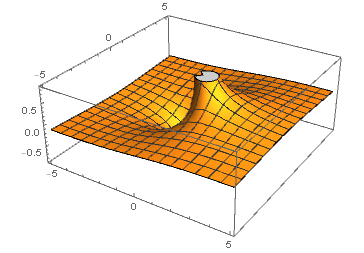
\includegraphics[scale=0.8]{image1.png}
			\end{figure}
		The above figure shows that the function $f(z)=1/z$ acts the way we expect along the real line. We can also see that the function is defined everywhere except for $z=0$, which makes good sense.
		
		\item Im$\left[f(z)\right] \rightarrow$ \codeword{Plot3D[Im[1/(x + I y)], {x, -5, 5}, {y, -5, 5}]}
		This code is identical to that above, but instead of plotting the real component of the inverse of $z$, we plot the imaginary component.
			\begin{figure}[H]
			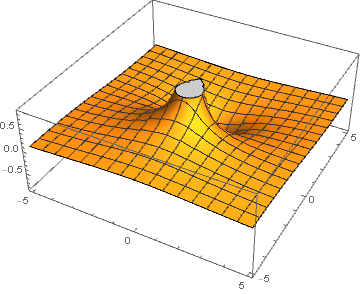
\includegraphics[scale=0.8]{image2.png}
			\end{figure}
		We can see from this graph that the it is identical to the real component except for it being rotated around the $z$-axis. This feels intuitive as on the complex plane, the imaginary numbers are "rotated" relative to the real line.
		
		\item $|f(z)| \rightarrow$ \codeword{Plot3D[Abs[1/(x + I y)], {x, -5, 5}, {y, -5, 5}]}
		Now we plot the magnitude of the inverses using the \codeword{Abs[]} function in Mathematica.
			\begin{figure}[H]
			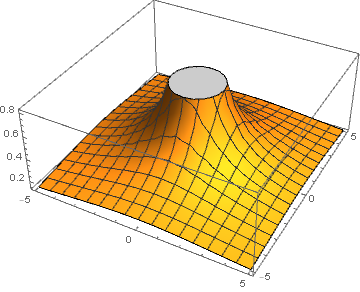
\includegraphics[scale=0.8]{image3.png}
			\end{figure}
		Nothing seen here is unexpected. Numbers closer to $0$ have extremely large inverses which naturally have a large positive magnitude. This causes the peak forming around the center of the figure.  
		
		\item Arg$f(z)\rightarrow$\codeword{Plot3D[Arg[1/(x + I y)], {x, -5, 5}, {y, -5, 5}]}
		This code shows the argument of the inverse of a complex numbers as the height of the graph.
			\begin{figure}[H]
			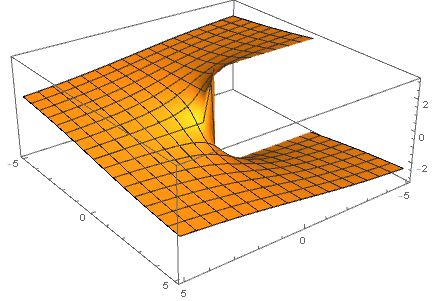
\includegraphics[scale=0.8]{image4.png}
			\end{figure}
		From this we are able to easily imagine the periodicity of the function by imagining this figure stacked on top of itself an infinite number of times. If you were to take a perfectly vertical line, it would intersect such a graph an infinite number of teams each corresponding to a $2\pi$ multiple of the argument. However, this graph only shows the principle branch of the argument which is inside the ragne $(-\pi,\pi]$.
	\end{enumerate}
	
	\item $f(z)=z^2-z$
	\begin{enumerate}
		\item $x=1,y-1,\text{ circle centered at } (1,1)$
		$f(z)=z^2-z$ can be rewritten as $f(x,y)=(x^2-y^2,2xy)-(x,y)=(x^2-y^2-x,2xy-y)$. The curves $x=1,y=1, \text{ and a circle of radius 2 centered at }(1,1)$ can be rewritten as $(1,t),(t,1),$ and $(2\cos{t}-1,2\sin{t}-1)$ respectively. By plugging these in to $f(x,y),$ we obtain the Mathematica code:
		\codeword{ParametricPlot[{{-t^2,t},{t^2-t-1,2t-1},{(2Cos[t]+1)^2-(2 Sin[t]+1)^2-(2Cos[t]+1),2(2Cos[t]+1)(2Sin[t]+1)-(2Sin[t]+1)}}, {t,-4.2,4.2}]}
			\begin{figure}[H]
			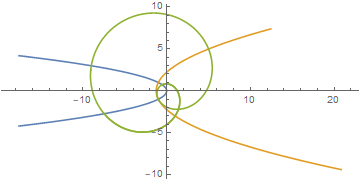
\includegraphics[scale=0.8]{image5.png}
			\end{figure}
		From this figure we can see that straight lines have been transformed into parabolas, which makes sense since the function has a $z^2$ term. What I find surprising is the image of the circle, shown above in green. It is still round, but has a crimp on one side where it meets the origin.
		\item The angles between intersections of graphs before and after the transformation are preserved. Thus, this function is a conformal map.
	\end{enumerate}
	
	\item Visualizing multi-valued function arg $z$.
	\begin{enumerate}
		\item $re^{i\theta} = r\cos{\theta}+i \: r\sin{\theta} \implies x=r\cos{\theta} \text{ and } y=r\sin{\theta}$.
		\item \codeword{ParametricPlot3D[{rCos[:theta:],rSin[:theta:],3:theta:},{:theta:,0,6 Pi},{r,0,10 Pi}]} produces the figure below. The multiplication of :theta: by 6 in the first set of curly brackets stretch the graph out to make the folds more visible. 
			\begin{figure}[H]
			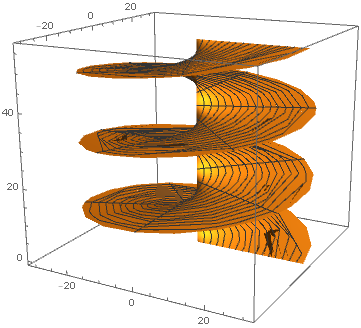
\includegraphics[scale=0.8]{image6.png}
			\end{figure}
		Here it is clear to see the periodicity of the non-principle arg$z$ function. If we were able to graph the function with parameters out to infinity, the entire space would be filled with this spiral around the center, with arms stretching out horizontally to an infinite distance. It would be a very disorienting place indeed.
	\end{enumerate}
	
	
	
	
\end{enumerate}
% ---------------------------------------------------
% Anything after the \end{document} will be ignored by the typesetting.
% ----------------------------------------------------

\end{document}

